\section{Introduction}
\vspace{-2mm}
On-policy distillation (OPD) has become a central technique for post-training large language models.
Recent systems like Qwen3~\citep{yang2025qwen3}, MiMo~\citep{xiao2026mimo}, and GLM-5~\citep{zeng2026glm} adopt OPD-style dense supervision in post-training pipelines. Thinking Machines Lab~\citep{lu2025onpolicydistillation} reports that an OPD recipe can reproduce strong reasoning gains at substantially lower compute than outcome-reward RL.
This makes OPD an attractive complement to supervised fine-tuning and verifiable RL: it supplies a token-level learning signal on long reasoning traces, rather than waiting for a sparse final-answer reward.

OPD's appeal lies in its on-policy nature. Off-policy distillation trains the student on fixed teacher-generated sequences, which induces the exposure-bias problem: at inference time, the student must act under prefixes that were not produced by the teacher or reference policy~\citep{bengio2015scheduled}.
OPD instead samples rollouts from the current student and evaluates the teacher on the same student-visited prefixes.
This design has also motivated recent self-distillation methods, where a model acts as its own teacher under privileged information or feedback and improves from its own on-policy experience~\citep{hubotter2026reinforcement,zhao2026self,shenfeld2026self}.
In long-horizon mathematical reasoning, this distinction matters: a single solution can contain thousands of tokens, so even small train-inference mismatches can compound across the trajectory.

However, the same on-policy design creates a new reliability problem.
The teacher is queried not only on prefixes where its local distribution offers useful corrections, but also on prefixes that have already drifted away from the teacher's reasoning process.
Recent OPD dynamics analysis points out that OPD success depends on local thinking-pattern compatibility and that reward quality can deteriorate with trajectory depth~\citep{li2026rethinking}.
We take this diagnosis as a design constraint: long-horizon OPD should not treat every generated token as equally worth supervising.

The missing piece is online reliability control.
Current OPD recipes usually choose a rollout budget before generation and then apply dense teacher rewards uniformly along the sampled response.
This creates a bad tradeoff.
A short fixed budget can discard useful long reasoning, while a long fixed budget spends substantial compute generating and scoring suffixes whose teacher signal may no longer be locally exploitable.
In practice, a single rollout can contain both regimes: an early prefix where student and teacher still share plausible next-token support, followed by a suffix where the student has committed to reasoning choices the teacher would not have taken.
What OPD needs is therefore not simply more or less dense reward, but a way to decide \emph{where} the dense reward is reliable enough to train on.

We propose \method, a reliability-aware modifier for long-horizon OPD that makes this decision during training.
Rather than filtering whole responses or imposing a fixed response length, \method~asks a position-level question: under the same student prefix, do the student and teacher still share a high-probability candidate region?
The primary signal is per-position top-$k$ overlap ratio, with teacher top-$p$/top-$k$ action acceptance as a stricter variant.
When the selected compatibility metric falls below its threshold, \method~records a prefix-drift event.
Cumulative drift events define a monotone reliability weight that attenuates later OPD rewards, and the same raw reliability signal defines an effective response length for dynamic rollout control.
The intended shift is from fixed-budget OPD to reliability-budgeted OPD: dense supervision should be allocated where the teacher remains actionable on the student's trajectory.

\begin{figure}[t]
\vspace{-3mm}
\centering
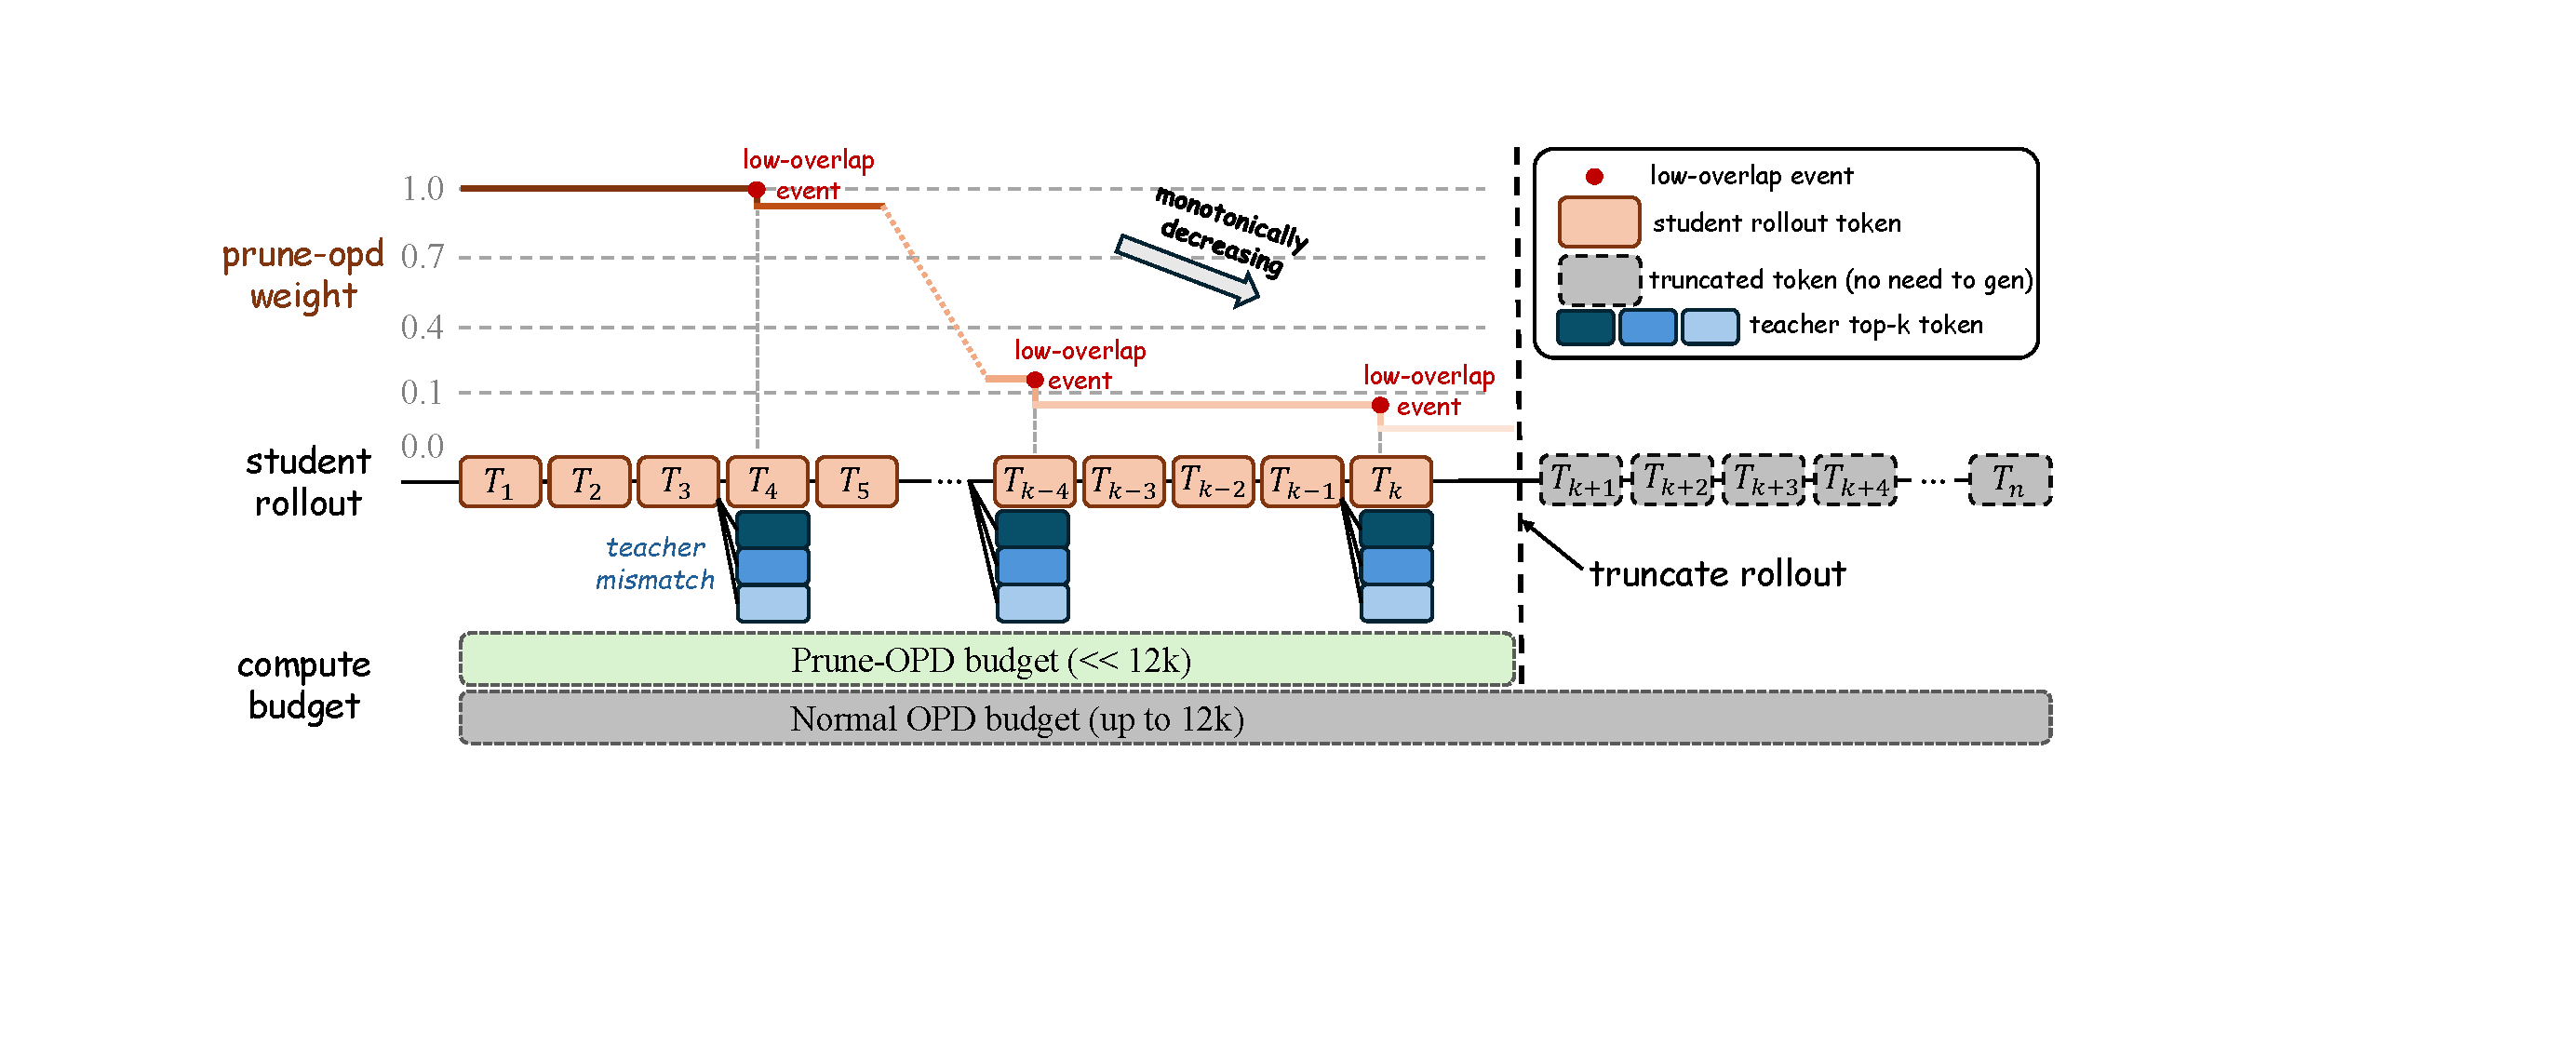
\includegraphics[width=\linewidth]{figs/main_compat.pdf}
\vspace{-1mm}
\caption{Conceptual overview of \method. \method~monitors local student-teacher compatibility along the student rollout, monotonically attenuates OPD rewards after low-overlap drift events, and truncates the response once reliable teacher supervision is exhausted.}
\label{fig:overview}
\vspace{-6mm}
\end{figure}

We conduct extensive experiments to evaluate whether reliability-aware pruning improves long-horizon OPD in practice.
The results validate the effectiveness of \method: it reduces training time by 37.6\%--68.0\% when dense supervision becomes unreliable, while preserving or improving downstream accuracy.
Additional runs show that the controller keeps long-context supervision when the reliability signal remains high, supporting the claim that \method~reallocates computation rather than blindly shortening rollouts. In summary, our contributions are:


\vspace{-2mm}
{\setlength{\leftmargini}{1.6em}
\begin{itemize}
    \item We formulate long-horizon OPD as a reliability-allocation problem on student-visited prefixes, connecting trajectory-depth degradation to local compatibility and reward exploitability.
    \item We propose \method, which converts cumulative prefix drift into monotone OPD reward attenuation and a dynamic response-length controller, without changing the baseline OPD path when disabled.
    \item We provide pilot evidence that reliability-aware pruning can reduce OPD training time by 37.6\%--68.0\% when prefix drift limits reliable supervision while preserving benchmark performance, and we specify fixed-length pruning controls to test whether the gains come from reliability rather than generic shortening.
\end{itemize}
}

